\chapter{Resultados}

\section{Métricas Obtenidas}

Para los resultados, se deben elaborar métricas que permitan determinar cuáles fueron los mejores algoritmos, es decir, los que presentan mejor desempeño según la experimentación determinada anteriormente. Primero se construyen las tablas que muestran los valores más relevantes en primera instancia, es decir, los errores en cada eje coordenado, sus promedios de error, varianzas y finalmente el \textit{root squared mean error}, o error cuadrático medio, el cual en términos euclidianos, representa la distancia de un punto a otro. La fórmula de este último es:

\begin{equation}
RMSE = \sqrt{\frac{1}{n} \sum_{j=1}^{n}(y_{j} - \hat{y_{j}})^{2}} 
\end{equation}

Para las tablas se considera el método dinámico y estático definido anteriormente. La \autoref{tabla-dinamica-nPCA} muestra los resultados obtenidos en el método dinámico sin utilizar PCA. Se debe considerar que todos los valores están en metros.


\begin{table}[ht!]
\centering
\caption[Resultados método dinámico sin  utilizar PCA]{Resultados método dinámico sin  utilizar PCA}
\label{tabla-dinamica-nPCA}
\begin{tabular}{|c|c|c|c|c|c|}
\hline
Clasificador & Error x & Error y & Varianza x & Varianza y & RMSE    \\ \hline
KNN          & 1.5858  & 4.6391  & 7.1970     & 2.1780     & 6.9323  \\ \hline
SVM          & 6.8207  & 2.8874  & 1.7243     & 0.5989     & 10.0323 \\ \hline
NN           & 4.3784  & 3.9113  & 13.0950    & 5.0712     & 8.2994  \\ \hline
\end{tabular}
\end{table}


Como muestra la \autoref{tabla-dinamica-nPCA}, los mejores resultados en términos generales son obtenidos por el método KNN, ya que los promedios en general son bajos, así como el RMSE. A pesar de esto, se debe notar que lo sigue Neural Network con un RMSE promedio de 8.2994 metros. 

La \autoref{tabla-dinamico-pca} muestra los resultados obtenidos por el método dinámico utilizando PCA.

\begin{table}[!ht]
\centering
\caption[Resultados método dinámico utilizando PCA con 5 componentes]{Resultados método dinámico utilizando PCA con 5 componentes}
\label{tabla-dinamico-pca}
\begin{tabular}{|c|c|c|c|c|c|}
\hline
Clasificador & Error x & Error y & Varianza x & Varianza y & RMSE   \\ \hline
KNN PCA      & 2.0023  & 4.3983  & 7.5113     & 2.0696     & 6.6812 \\ \hline
SVM PCA      & 6.8948  & 2.4257  & 4.1134     & 2.0348     & 9.5668 \\ \hline
NN PCA       & 5.8874  & 4.4513  & 8.6088     & 3.2089     & 9.5188 \\ \hline
\end{tabular}
\end{table}

En este caso, los resultados son ligeramente mejores en términos de RMSE, lo cual indica que PCA si puede eliminar parte de la correlación espacial e información repetida dentro de los datos. En este caso nuevamente KNN con PCA obtiene el mejor resultado, seguido por Neural Network y finalmente SVM. Las varianzas de cada eje igualmente son relativamente altas, por lo que esto puede afectar mucho el posicionamiento en general, ya que, a mayor varianza, más error durante el tiempo se presenta, y más alejados están los valores desde el promedio.

Para la siguiente tabla, ahora se considera el método estático, el cual como se ha descrito, mide la posición al estar estático en un determinado lugar. 

\begin{table}[!h]
\centering
\caption[Resultados método estático sin utilizar PCA]{Resultados método estático sin utilizar PCA}
\label{tabla-estatica}
\begin{tabular}{|c|c|c|c|c|c|}
\hline
Clasificador & Error x & Error y & Varianza x & Varianza y & RMSE   \\ \hline
KNN          & 3.2385  & 1.5417  & 3.3321     & 1.0940     & 5.0520 \\ \hline
SVM          & 5.2493  & 1.6986  & 2.0598     & 0.7594     & 7.0241 \\ \hline
NN           & 3.7300  & 2.1937  & 5.8885     & 0.7373     & 4.4857 \\ \hline
\end{tabular}
\end{table}

Para este caso, la \autoref{tabla-estatica}, muestra que ahora los mejores resultados son obtenidos por el método Neural Networks con un RMSE de 4.4857 en promedio. Para todos los algoritmos, las varianzas se ven reducidas sustancialmente, lo que es esperable debido a que, al estar estático en una posición, las ondas electromagnéticas no se ven alteradas o cambiantes a través del tiempo, lo cual estabiliza la señal recibida por los Beacons. Para este caso, primero es NN, luego KNN y finalmente SVM en términos de RMSE. Igualmente, los valores de error obtenidos son muy altos para lograr un posicionamiento exacto.

Por último, las métricas obtenidas para el posicionamiento estático utilizando PCA se muestran a continuación.

\begin{table}[!h]
\centering
\caption[Resultados método estático utilizando PCA con 5 componentes]{Resultados método estático utilizando PCA con 5 componentes}
\label{estatico-pca}
\begin{tabular}{|c|c|c|c|c|c|}
\hline
Clasificador & Error x & Error y & Varianza x & Varianza y & RMSE   \\ \hline
KNN PCA      & 2.9892  & 1.4475  & 3.1487     & 1.6391     & 5.0340 \\ \hline
SVM PCA      & 3.2313  & 1.4905  & 3.0630     & 1.7817     & 5.1757 \\ \hline
NN PCA       & 1.5578  & 1.7488  & 3.8045    & 2.6885     & 3.9341 \\ \hline
\end{tabular}
\end{table}
 
La \autoref{estatico-pca} muestra mejores resultados para todos los clasificadores, disminuyendo así los valores totales. Esto muestra nuevamente que mediante la técnica PCA es posible reducir el error. Por otra parte, las varianzas permanecen pequeñas a excepción de Neural Network. El mejor resultado es obtenido por Neural Network con PCA con un error promedio de 3.9341 metros, seguido por KNN PCA y finalmente SVM PCA.

El siguiente análisis realizado, tiene que ver con el valor de \textit{Cumulative distribution function}, el cual está definido como el valor de una variable aleatoria $X$, o su función de distribución, que al ser evaluada en $x$, es la probabilidad que $X$ tome valores menores o iguales a $x$, Esta función está definida matemáticamente como:

\begin{equation}
F_{X} (x) = P(X \le x)
\end{equation}

La importancia de este indicador es que refleja en este caso, que tan frecuente se repite un valor de error, o, dicho de otra forma, en qué porcentaje se puede asegurar que el error será menor o igual a un determinado valor, por ejemplo el 90\% de las veces el error es menor a 10 metros. Con esta definición, a continuación, se procede a mostrar los gráficos obtenidos tanto para el método estático como para el método dinámico. La \autoref{fig:cdf-dinamicos} muestra esta situación.

\newpage

\begin{figure}[ht!]
\centering
\begin{subfigure}{.5\textwidth}
  \centering
  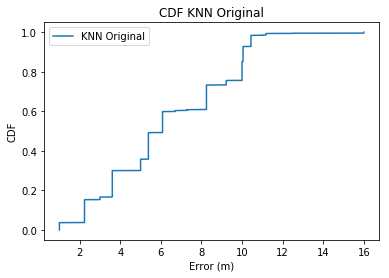
\includegraphics[width=.8\linewidth]{figures/cdf-knn-dinamico.png}
  \caption{CDF KNN}
  \label{fig:sub1}
\end{subfigure}%
\begin{subfigure}{.5\textwidth}
  \centering
  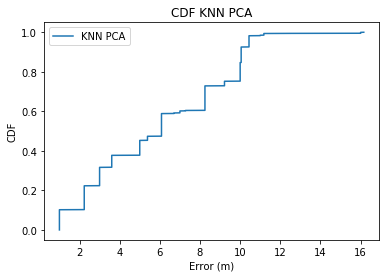
\includegraphics[width=.8\linewidth]{figures/cdf-knnPCA-dinamico.png}
  \caption{CDF KNN PCA}
  \label{fig:sub2}
\end{subfigure}

\begin{subfigure}{.5\textwidth}
  \centering
  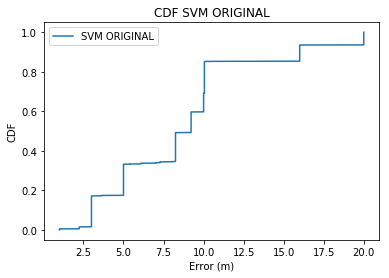
\includegraphics[width=.8\linewidth]{figures/cdf-svm-dinamico.png}
  \caption{CDF SVM}
  \label{fig:sub1}
\end{subfigure}%
\begin{subfigure}{.5\textwidth}
  \centering
  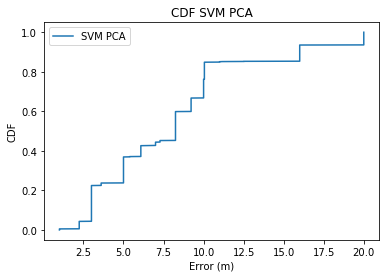
\includegraphics[width=.8\linewidth]{figures/cdf-svmPCA-dinamico.png}
  \caption{CDF SVM PCA}
  \label{fig:sub2}
\end{subfigure}

\begin{subfigure}{.5\textwidth}
  \centering
  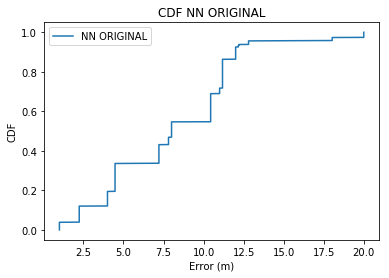
\includegraphics[width=.8\linewidth]{figures/cdf-nn-dinamico.png}
  \caption{CDF NN}
  \label{fig:sub1}
\end{subfigure}%
\begin{subfigure}{.5\textwidth}
  \centering
  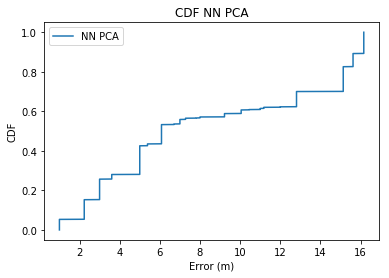
\includegraphics[width=.8\linewidth]{figures/cdf-nnPCA-dinamico.png}
  \caption{CDF NN PCA}
  \label{fig:sub2}
\end{subfigure}
\caption[Cummulative distribution function para el método dinámico]{Cummulative distribution function para el método dinámico obtenido utilizando los distintos algoritmos \\
{\scriptsize (Fuente: Elaboración Propia)}}
\label{fig:cdf-dinamicos}
\end{figure}

Los gráficos muestran que los valores son muy símiles en cuanto a si se utiliza PCA o no. K-NN se mantiene el 80\% de las veces bajo los 10 metros, en ambos casos y cerca del 60\% bajo los 6 metros. Por otro lado, SVM igualmente el 80\% de las veces está bajo los 10 metros con respecto a SVM sin utilizar PCA, el 50\% de las veces está bajo los 8 metros y utilizando PCA esto ocurre el 60\% de las veces por lo que PCA es más estable en este sentido, y genera valores más uniformes. Finalmente, con las redes neuronales, los resultados presentados sin utilizar PCA, el 80\% de las veces esta cercano a los 12 metros y 50\% de las veces en los 7.5 metros. Utilizando PCA en este último caso, los resultados son mejores para porcentajes más bajos, ya que el 80\% de las veces esta sobre los 15 metros aproximadamente,  pero esto no cambia relativamente hacia porcentajes superiores, sin embargo para porcentajes inferiores los valores mejoran, ya que por ejemplo para un error menor a 6 metros, ocurre con una probabilidad del 60\% .

Para ver el mínimo error al 100\%, es decir, el error mínimo que está asegurado, se realiza la \autoref{cambio-cdf-dinamico} comparando sus valores utilizando o no PCA. Nuevamente los valores están en metros.

\newpage

\begin{table}[!h]
\centering
\caption[Error con un CDF del 100 \% para los algoritmos analizados  en el método dinámico]{Error con un CDF del 100 \% para los algoritmos analizados  en el método dinámico}
\label{cambio-cdf-dinamico}
\begin{tabular}{|c|c|c|c|}
\hline
Clasificador & Sin PCA & Con PCA & Mejora     \\ \hline
KNN          & 16.576  & 16.1554 & 2.5374 \%  \\ \hline
SVM          & 20.8962 & 19.3874 & 7.2204 \%  \\ \hline
NN           & 20.5677 & 16.1554 & 21.4525 \% \\ \hline
\end{tabular}
\end{table}


Como se observa en la tabla \autoref{cambio-cdf-dinamico}, todos los valores son mejorados utilizando PCA, además los errores menores se obtienen con NN y KNN, aunque KNN es más estable ya que con y sin PCA presenta valores semejantes.

Para el método estático se realiza el mismo análisis. Los gráficos obtenidos para el error CDF son los siguientes:

\begin{figure}[ht!]
\centering
\begin{subfigure}{.5\textwidth}
  \centering
  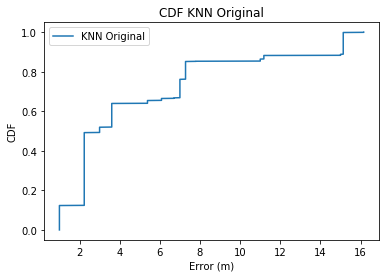
\includegraphics[width=.8\linewidth]{figures/cdf-knn-estatico.png}
  \caption{CDF KNN}
  \label{fig:sub1}
\end{subfigure}%
\begin{subfigure}{.5\textwidth}
  \centering
  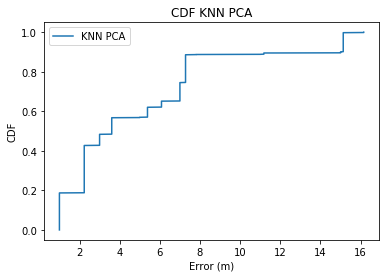
\includegraphics[width=.8\linewidth]{figures/cdf-knnPCA-estatico.png}
  \caption{CDF KNN PCA}
  \label{fig:sub2}
\end{subfigure}

\begin{subfigure}{.5\textwidth}
  \centering
  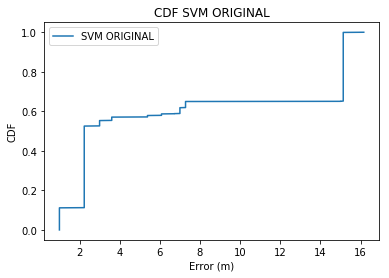
\includegraphics[width=.8\linewidth]{figures/cdf-svm-estatico.png}
  \caption{CDF SVM}
  \label{fig:sub1}
\end{subfigure}%
\begin{subfigure}{.5\textwidth}
  \centering
  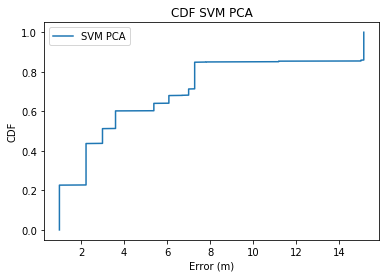
\includegraphics[width=.8\linewidth]{figures/cdf-svmPCA-estatico.png}
  \caption{CDF SVM PCA}
  \label{fig:sub2}
\end{subfigure}

\begin{subfigure}{.5\textwidth}
  \centering
  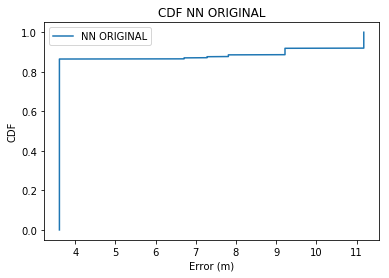
\includegraphics[width=.8\linewidth]{figures/cdf-nn-estatico.png}
  \caption{CDF NN}
  \label{fig:sub1}
\end{subfigure}%
\begin{subfigure}{.5\textwidth}
  \centering
  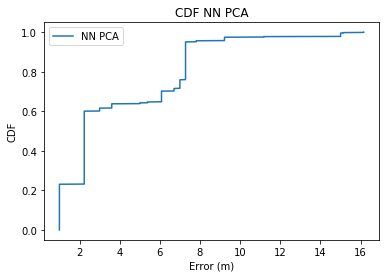
\includegraphics[width=.8\linewidth]{figures/cdf-nnPCA-estatico.png}
  \caption{CDF NN PCA}
  \label{fig:sub2}
\end{subfigure}
\caption[Cummulative distribution function para el método estático]{Cummulative distribution function para el método estático obtenido utilizando los distintos algoritmos \\
{\scriptsize (Fuente: Elaboración Propia)}}
\label{fig:cdf-estaticos}
\end{figure}

Los gráficos para los casos estáticos muestran de manera general que los resultados son mucho mejores, esto es esperable debido a como se discute anteriormente, al estar estático es mucho más estable la señal y por ello se obtienen mejores valores de CDF. Para KNN, el error a los 8 metros se mantiene con una probabilidad de sobre el 80\%, lo cual representa una mejora aproximada de 2 metros respecto al método dinámico. Utilizando PCA se mantiene la tendencia, además se debe observar que para un error menor o igual a 4 metros, ocurre con probabilidad de 60\% lo cual es una mejora significativa.

Para SVM, aunque el error es muy grande en general, se debe tener en cuenta que con cerca del 50\% de las veces, el error esta cercano a los 2 metros. Para SVM con PCA los resultados son muy similares al método dinámico. Finalmente, para las redes neuronales, ocurre un comportamiento distinto a los anteriormente vistos, ya que la probabilidad de que el error sea menor o igual a 2 metros sobrepasa el 80\%, es decir esta siempre muy cercano a la posición verdadera. Esto indica que NN estático es muy estable, a diferencia de lo que ocurre con este mismo algoritmo en el método dinámico. Con respecto a NN con PCA, es claro que no existe mejora con respecto al caso sin PCA, de hecho, empeora el desempeño. Esto puede deberse a factores que serán explicados posteriormente, con respecto a las propiedades de las redes neuronales. Lo que se debe tener en cuenta es que la probabilidad de un error menor a 8 metros es cercana al 90\%, y el 60\% de las veces el error es menor a 2 metros, para NN con PCA.

La tabla del error mínimo al 100\% de CDF se muestra a continuación:

\begin{table}[!h]
\centering
\caption[Error con un CDF del 100 \% para los algoritmos analizados  en el método estático]{Error con un CDF del 100 \% para los algoritmos analizados  en el método estático}
\label{cambio-cdf-estatico}
\begin{tabular}{|c|c|c|c|}
\hline
Clasificador & Sin PCA  & Con PCA & Cambio    \\ \hline
KNN          & 16.1554  & 16.1554 & 0 \%      \\ \hline
SVM          & 16.1554  & 15.1327 & 6.33 \%   \\ \hline
NN           & 11.18033 & 16.1554 & -44.49 \% \\ \hline
\end{tabular}
\end{table}

Los cambios para KNN y SVM no son significativos, y además los errores mínimos son muy similares, del orden de los 16 metros, lo cual indica que PCA funciona efectivamente para reducir la información redundante. Con respecto a NN, se presenta una anomalía al utilizar o no PCA, esto se debe a que las redes neuronales ya hacen una reducción de la dimensionalidad en sus capas escondidas, y retienen lo mejor de la información en cada paso, por lo que aplicar PCA no ayuda demasiado, debido a que resta información relevante, entonces, para Neural Networks, específicamente deep learning, PCA no es efectivo, y es mejor pasar la mayor cantidad de información \textbf{relevante} que se posea.

El siguiente análisis tiene relación con la dispersión del error, vale decir, que tan distintos son los valores, y además determinar en qué valores se agrupan en su mayoría los datos. Para ello se utiliza un análisis de diagrama de cajas o \textit{boxplot}. Con este tipo de análisis se puede visualizar la dispersión y distribución de los datos en términos de cuartiles. En primer lugar, se construyen las siguientes tablas que muestran los valores relevantes para el boxplot. La \autoref{tabla-boxplot-dinamico} resume los valores de error obtenidos para el método dinámico.

\begin{table}[!ht]
\centering
\caption[Tabla Boxplot método dinámico]{Tabla resumen de los valores necesarios obtenidos para construir el Boxplot del método dinámico}
\label{tabla-boxplot-dinamico}
\begin{tabular}{|c|c|c|c|c|c|c|c|c|}
\hline
\textbf{Clasificador} & \textbf{Mediana} & \textbf{25\%} & \textbf{75\%} & \textbf{90\%} & \textbf{95\%} & \textbf{IQR} & \textbf{Min} & \textbf{Max} \\ \hline
KNN                   & 6.0827           & 3.6055        & 9.2195        & 10.0498       & 10.4403       & 5.6139       & 0.0            & 16           \\ \hline
KNN PCA               & 6.0827           & 3.0           & 9.2195        & 10.0498       & 10.4403       & 6.2195       & 0.0          & 16.1554      \\ \hline
SVM                   & 9.2195           & 5.0           & 10.0498       & 16.0          & 20.0          & 5.0498       & 0.0          & 16.0         \\ \hline
SVM PCA               & 8.2462           & 5.0           & 10.0          & 16.0          & 20.0          & 5.0          & 0.0          & 16.0         \\ \hline
NN                    & 8.0              & 4.4721        & 11.1803       & 12.0          & 12.8062       & 6.7082       & 0.0          & 20.0         \\ \hline
NN PCA                & 6.0827           & 3.0           & 15.1327       & 16.1554       & 16.1554       & 12.1327      & 0.0          & 16.1554      \\ \hline
\end{tabular}
\end{table}


Para el método estático, la \autoref{tabla-boxplot-estatico} muestra los valores resultantes de error.

\newpage

\begin{table}[!ht]
\centering
\caption[Tabla Boxplot método estático]{Tabla resumen de los valores necesarios obtenidos para construir el Boxplot del método estático}
\label{tabla-boxplot-estatico}
\begin{tabular}{|c|c|c|c|c|c|c|c|c|}
\hline
\textbf{Clasificador} & \textbf{Mediana} & \textbf{25\%} & \textbf{75\%} & \textbf{90\%} & \textbf{95\%} & \textbf{IQR} & \textbf{Min} & \textbf{Max} \\ \hline
KNN                   & 3.0              & 2.2360        & 7.0           & 15.1327       & 15.1327       & 4.7639       & 0.0          & 11.1803      \\ \hline
KNN PCA               & 3.6055           & 2.2360        & 7.2801        & 15.0          & 15.1327       & 5.0440       & 0.0          & 11.1803      \\ \hline
SVM                   & 2.2360           & 2.1604        & 15.1327       & 15.1327       & 15.1327       & 12.9723      & 0.0          & 16.1554      \\ \hline
SVM PCA               & 3.0              & 2.1604        & 7.2801        & 15.1327       & 15.1327       & 5.1197      & 0.0          & 11.1803      \\ \hline
NN                    & 3.6055           & 3.6055        & 3.6055        & 9.2195        & 11.1803       & 0.0          & 3.6055       & 3.6055       \\ \hline
NN PCA                & 2.2360           & 2.4053        & 7.0           & 7.2801        & 7.2801        & 4.7639       & 0.0          & 11.1803      \\ \hline
\end{tabular}
\end{table}

Finalmente, el diagrama de cajas es el siguiente:

\begin{figure}[ht!]
\centering
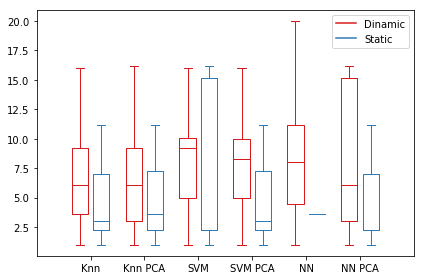
\includegraphics[width=.6\textwidth]{figures/boxplot.png}
\caption[Diagrama de cajas para método estático y dinámico]{Diagrama de cajas para método estático y dinámico \\
{\scriptsize (Fuente: Elaboración Propia)}}
\label{fig:boxplot}
\end{figure}

La \ref{tabla-boxplot-dinamico} y \ref{tabla-boxplot-estatico} muestran los valores resultantes. Se debe tener en cuenta que los valores son iguales o muy similares cuando se utiliza PCA con el algoritmo original, debido a que la distribución de los datos es idéntica y el algoritmo es el mismo, además como se menciona anteriormente, los valores no cambian significativamente lo cual hace que PCA mantenga la distribución original y no cambie demasiado sus valores.

Se debe notar que muchas veces se repiten los valores de mediana o los cuartiles, por ejemplo, entre distintos algoritmos, sobre todo para el método estático. Esto puede deberse a la gran cantidad de datos.

Por último, antes de analizar en términos generales los resultados, se procede a mostrar las diferencias temporales existentes, es decir, los incrementos referentes a la técnica PCA. La \autoref{tiempo-tabla} muestra estos resultados en términos de milisegundos y la respectiva mejora.


\begin{table}[ht!]
\centering
\caption[Mejoras de tiempo en cada algoritmo]{Mejoras de tiempo en cada algoritmo al usar la técnica PCA para reducir la dimensionalidad}
\label{tiempo-tabla}
\begin{tabular}{|c|c|c|c|}
\hline
\textbf{Clasificador} & \textbf{Sin PCA} & \textbf{Con PCA} & \textbf{Incremento} \\ \hline
KNN                   & 64.9642          & 59.6786          & 8.1361\%            \\ \hline
SVM                   & 54.5985          & 25.6085          & 53.0966\%           \\ \hline
NN                    & 0.7610           & 0.5777           & 24.0867\%           \\ \hline
\end{tabular}
\end{table}



\section{Análisis de resultados}

A partir de los resultados obtenidos, se hace el análisis de los mejores algoritmos para el posicionamiento indoor según los parámetros y proceso de experimentación propuesto. Lo primero que se debe tener en consideración son los errores medios, ya que este parámetro afecta directamente al posicionamiento y es uno de los más relevantes al momento de seleccionar el mejor algoritmo. Con respecto al método dinámico, la \autoref{tabla-dinamica-nPCA} muestra que el mejor valor es obtenido por KNN con un RMSE de 6.9323 metros, seguido de NN con 8.2994 metros y finalmente SVM con 10.0323. Estos valores reflejan que en este caso KNN sería la mejor opción, sin embargo el error es demasiado grande como para lograr un posicionamiento exacto en los tres casos. Con respecto a la tabla \ref{tabla-dinamico-pca}, esta muestra resultados similares, en este caso KNN nuevamente se impone ante los demás clasificadores, con un error promedio de 6.6812 metros, seguido de redes neuronales con 9.5188 metros y SVM con 9.5668 metros. Se debe tener en cuenta que las varianzas de cada eje coordenado son altas, sobre todo en el eje $x$, por lo que esto repercute negativamente al momento del posicionamiento y de obtener el error medio \textbf{RMSE}. Tomando en consideración los resultados del método dinámico con y sin PCA, claramente KNN es la opción para este tipo de método, en donde existen cambios espaciales, por lo que este no se ve afectado en demasía por la posición en donde es tomada la medición. Esto se debe principalmente a que para KNN es irrelevante los datos de entrada, ya que siempre realiza una búsqueda completa y debe analizar cada punto, por lo que evidentemente puede obtener mejores valores, pero su procesamiento demora más. Además, es mejor utilizar PCA, sobre todo para KNN, así se reduce la información irrelevante y el algoritmo realiza menos iteraciones, lo cual es sinónimo de menos tiempo de computo, además que disminuye el error, aunque es en una pequeña fracción de 0.25 metros.

Realizando el mismo análisis para el caso del método estático, los resultados indican que los menores valores de error se obtienen utilizando redes neuronales o deep learning, con un error promedio de 4.4857 metros, seguido de 5.0520 metros y finalmente SVM con 7.0241 metros. Las varianzas en este caso son mucho más pequeñas, por lo que los resultados son mucho más estables, lo cual es esperable, ya que no hay movimiento efectivo, por lo que solo afecta el cambio en el entorno y la temporalidad. Por otra parte, el error en cada eje es mucho menor que el método dinámico, lo cual se refleja en el error promedio. A pesar de que el error disminuye, 4 metros aún es demasiado error para posicionamiento exacto, pero se debe recordar que este es un problema de clasificación y para obtener la posición exacta se debe acertar perfectamente en la clasificación y en este caso, la grilla al ser de $4 \times 4$ metros, si se falla en la clasificación aunque sea en 1 unidad relativa en la posición, es decir, la clase adyacente, el error ya es de al menos 4 metros, por lo mismo, no es sorpresivo encontrar errores tan altos. 

Con respecto al método estático utilizando PCA, nuevamente los errores decrecen en todos los algoritmos, al igual que el error en cada eje y la varianza. Esto demuestra que utilizar PCA es una buena opción si solo se analiza el error promedio. La mejora de las redes neuronales es de 0.55 metros, lo cual es significativo, considerando además que PCA ayuda a reducir el tiempo de procesamiento. El objetivo del método estático es evaluar la estabilidad temporal de los algoritmos, y el que obtiene el mejor resultado es NN, esto se debe a que las redes neuronales no son afectadas mayormente por los cambios del entorno, es decir, el ruido, porque puede reconocer estos patrones espaciales y temporales, y al estar estático mucho tiempo, no se ve mayormente influenciado, por lo que logra determinar de mejor manera la clasificación respectiva. Entonces, para el método estático es mejor utilizar NN con PCA.

Ya que fueron analizadas las métricas básicas, se prosigue a analizar el CDF. Como se menciona anteriormente en general los resultados para el método estático y dinámico son muy similares al momento de analizar el CDF como muestran los gráficos \ref{fig:cdf-dinamicos} y \ref{fig:cdf-estaticos}. A modo de síntesis, se debe tener claro que la mayor cantidad de las veces, aproximadamente el 80\%, el error es menor a 10 metros , y el 60\% de las veces es menor a 8 metros para el método dinámico. Porcentajes menores a estos no son relevantes, ya que no es muy frecuente y tampoco indica valores fiables. Con lo anterior en mente, se debe notar que la mejor curva de CDF para el método dinámico es obtenida por el algoritmo KNN, seguido por SVM y finalmente redes neuronales. Claramente, se ve una distorsión en las redes neuronales al utilizar PCA, que afecta el valor del CDF y su respectivo error, por lo demás los gráficos son muy similares en su forma. Lo que se busca en este tipo de graficas de error, es curvas muy empinadas para valores pequeños de error, ya que esto significa que la probabilidad de obtener estos valores pequeños es muy alta, por lo que la confianza en el algoritmo aumenta, y en este caso todas las formas de las gráficas son diagonales, a excepción de NN con PCA que es mucho más achatada, lo cual indica que para una determinada probabilidad, el error incrementa mucho, lo cual no es bueno para el algoritmo y lo convierte en poco fiable.

Respecto al CDF de 100\%, es decir, lo que siempre ocurrirá para el método dinámico, el error mínimo que se alcanza sin PCA es presentado por KNN con 16.576 metros y al utilizar PCA, este valor disminuye a 16.1554 metros, obteniendo así una mejora de 2.5375\%.  Se debe destacar que el error de redes neuronales con PCA disminuye de 20.5677 a 16.1554 metros, esto es 21.4525\%, que es muy alto, lo que significa que NN con PCA a pesar de ser menos estable y tener mayores errores para porcentajes más bajos(es menos fiable), aun así el error mínimo esperable es mucho mejor que el error mínimo esperable sin utilizar PCA, es decir, mucho mejores valores pero con menos estabilidad en estos. Dicho todo lo anterior, KNN es el claro ganador cuando se analiza CDF para el método dinámico, sobre todo considerando PCA, lo cual es idéntico a lo determinado en el apartado anterior de análisis de error medio o RMSE.

Para el análisis de CDF en el caso estático, los resultados son mucho mejores comparados al caso del método dinámico como era esperable, debido a la estabilidad de las ondas emitidas. Aquí se hace un análisis de cada algoritmo debido a que son resultados muy distintos entre ellos. En primer lugar, KNN tiene errores menores o iguales a 8 metros con una probabilidad de 80\% aproximadamente, y de 4 metros con una probabilidad de 60\%. Por otra parte, cuando se aplica PCA los resultados son idénticos, esto incluso se puede verificar con la forma de las curvas como muestra el grafico \ref{fig:cdf-estaticos}. Respecto a SVM, cuando no se aplica PCA, la curva es muy achatada y el error de 15 metros con una probabilidad de 60\%, lo cual es muy malo. Cuando se adopta SVM con PCA este error disminuye significativamente, con un error de 8 metros con probabilidad de 80\% y de aproximadamente 4 metros con probabilidad de 60\%. Finalmente, cuando se analizan las redes neuronales ocurre una anomalía, ya que el error decrece a 2.5 metros con una probabilidad mayor a 80\%, lo que es una mejora muy significativa y relevante. Esto puede deberse a lo que se menciona anteriormente, las propiedades de mantener el ruido fuera y ser estable temporalmente, es decir, no ser muy influenciado por cambios a través del tiempo. Por otra parte, al aplicar PCA a NN, el error aumenta, llegando como los otros algoritmos a aproximadamente 8 metros con probabilidad mayor al 80\%. Con lo anterior, es claro que redes neuronales es el ganador en este análisis, seguido de KNN y SVM. Es necesario recalcar que PCA no es necesario y que afectaría en este caso los resultados, lo cual no es coincidente con lo obtenido en el análisis de error medio, y esto es perfectamente válido, ya que el CDF muestra solo la probabilidad de que el error sea menor a cierto valor, es por ello que ayuda a tomar la decisión de utilizar o no PCA. 

Para el análisis del CDF al 100\%, la \autoref{cambio-cdf-estatico}, muestra que KNN no cambia prácticamente, SVM disminuye 16.1544 a 15.1327 metros, disminuyendo así 6.33\%. Finalmente, las redes neuronales pasan de 11.18033 metros sin PCA a 16.1554 metros con este, lo cual supone un aumento de 44.49\%.  Los resultados muestran los errores mínimos asociados. En este caso y como se menciona anteriormente, NN con PCA aumenta el error, mientras SVM con kernel Gaussiano mejora un poco, aunque no siempre ocurrirá esto, ya que PCA origina un espacio no correlacionado y SVM con función de radio basal asume que el espacio se distribuye de manera Gaussiana, lo cual no siempre es cierto, y por lo que tener en cuenta esta mejora tanto para el caso estático y dinámico no es fiable, debido a que puede ser producto de una casualidad. Con lo anterior, es claro que para el método estático es mejor utilizar redes neuronales sin PCA basado en el análisis del CDF.

Para el análisis de distribución de los datos, es necesario analizar los datos relativos a los percentiles o cuartiles, y el análisis cualitativo del diagrama de cajas.  Con respecto a los datos de la \autoref{tabla-boxplot-dinamico}, que representan la distribución obtenida en el método dinámico, se observa que la mediana de los errores se encuentra entre los valores 6.0827 metros y 9.2195 metros. Por otra parte, para el primer cuartil, es decir, $Q1$, que es equivalente al 25avo percentil, el máximo valor es 5 metros en SVM y SVM utilizando PCA, y el mínimo lo obtiene redes neuronales con PCA, con 3 metros, lo cual es indicativo que el 25\% menor de los datos están en este rango, por lo que no es buen indicativo para el posicionamiento, debido a que este error es muy grande. Luego, el tercer cuartil, es decir $Q3$, esta entre 9.2195 metros para KNN y KNN PCA, hasta 15.1327 para NN PCA. Esto indica que la distribución del 50\% total de los datos está en un rango intercuartílico (Q3 – Q1) de 5.0 metros para SVM PCA en el mejor caso, y 12.1327 metros para el peor caso. 

Con lo anterior, es claro que el mejor algoritmo según este análisis es KNN PCA, debido a que sus valores de $Q1$ y $Q3$ son los más bajos y el rango intercuartílico es no es tan grande, por lo que se puede determinar que el valor máximo de la distribución no escapa tanto, en este caso es 16 metros, que se condice con los análisis de CDF. Los peores resultados en la distribución del error lo obtienen las redes neuronales siempre y cuando se analicen solo los datos del Boxplot, ya que si se toman en cuenta los percentiles 90 y 95, SVM es el peor debido a que alcanza los 20 metros en el 95\% inferior de los datos. El peor valor entonces, según el Boxplot es obtenido por NN PCA, ya que el tercer cuartil es muy elevado, además su rango intercuartílico es muy grande, lo que indicaría que el 50\% central de los datos están demasiado dispersos en este rango, y a pesar de que su distribución general es similar a las demás, ya que el mínimo y máximo están en un rango parecido a KNN por ejemplo, la distribución interna es muy disociada, mostrando así falta de agrupación en los datos, provocando de esta forma resultados poco estables.

Con respecto a la \autoref{tabla-boxplot-estatico}, en este caso la mediana disminuye considerablemente con respecto al caso dinámico, lo cual es un indicativo de que la distribución de los datos tiende a estar mucho más cercanos a valores de error menor. Luego, el primer cuartil muestra como los datos se agrupan en valores muy cercanos a 2 metros, a excepción de las redes neuronales sin utilizar PCA, la cual es 3.6055 metros. Continuando con el análisis, para el tercer cuartil, el menor valor es obtenido por las redes neuronales sin PCA, esto como se ha mencionado anteriormente en los análisis de las métricas, es una anomalía, ya que como se observa en la tabla, el primer y tercer cuartil coinciden, lo cual se traduce en un rango intercuartílico igual a cero, vale decir, se asegura que al menos el 50\% de los datos corresponden exactamente a este valor de error, 3.6055 metros, inclusive el valor mínimo y máximo coinciden en este valor, con lo cual se puede establecer que la gran mayoría de los datos de error obtenidos por NN determinaron la misma posición, es por ello que el error se repite y la distribución es uniforme, a excepción de los \textit{outlayers} fuera del rango. Posteriormente, la menor distribución es la de NN con PCA, aunque es idéntica a la presentada por KNN, su mediana es mucho más baja y por otra parte al mirar los percentiles 90 de ambas distribuciones, NN con PCA alcanza los 7.2801 metros, mientras que KNN y KNN con PCA obtienen valores sobre los 15 metros, por lo que la diferencia es muy alta. Finalmente, SVM, a pesar de tener una mediana muy baja, su cuartil 3 es muy alto, lo que implica una distribución muy dispersa sobre el 50\% de los datos centrales, lo que no es bueno por ser demasiado variable, por otra parte, su valor máximo es el más alto, con 16.1554 metros. Finalmente, SVM con PCA logra mejores resultados, sin embargo, su mediana y rango intercuartílico son más grandes que en los otros casos, por lo que queda resegado a la última posición en términos de distribución.

A continuación se analiza el \autoref{fig:boxplot}, para realizar además un análisis cualitativo. Como se observa en el gráfico, para el caso dinámico (diagramas de caja rojos), KNN y KNN con PCA muestran una distribución estable, y con sus valores mínimos y máximos no muy alejados del 50\% de los datos, seguido posteriormente de SVM y SVM PCA, con un rango intercuartílico estable y pequeño. Estos análisis demuestran que, para los dos algoritmos, la técnica PCA no ayuda demasiado a mejorar los resultados. Finalmente, las redes neuronales, a pesar de las métricas obtenidas en análisis anteriores, acá la distribución es peor, y sus valores de error son más altos, sobre todo en redes neuronales con PCA, en donde el rango intercuartílico es muy grande y la mayor parte de los datos están allí, aunque si bien la mediana es baja, la parte superior de los datos posee errores muy altos, por lo que se torna muy poco estable y los errores muy dispersos.

Respecto al método estático, KNN muestra exactamente el mismo comportamiento, solo que esta vez los errores están por debajo del método dinámico, mientras que en este caso es seguido por redes neuronales con un error y una distribución orientada a valores más bajos. Aquí se muestra la anomalía de la red neuronal sin PCA, en donde se obtiene un mismo resultado todo el tiempo, por lo que es muy estable en sus valores, mientras que al utilizar PCA empeoran los resultados por los motivos explicados anteriormente, en donde las redes neuronales, específicamente deep learning es mucho mejor utilizar los datos completos y que sea el mismo algoritmo el que determina las mejores componentes. SVM por su parte, al no utilizar PCA muestra un rango de valores muy altos, por lo que esta información redundante repercute negativamente cuando las pruebas se realizan por mucho tiempo en una posición estática, por lo que en este caso es mejor realizar PCA para determinar las componentes más favorables, ya que al tener información no relevante, SVM puede verse afectado por sus márgenes y restricciones propias, y pequeños cambios en las ondas electromagnéticas, provoca una mala clasificación, y esto se refleja cuando el tiempo de experimentación es largo.

Finalmente, se debe analizar las diferencias en el tiempo de procesamiento, ya que este es un valor fundamental para tomar una decisión en la elección del mejor algoritmo. Para ello se analiza la \autoref{tiempo-tabla}, la cual muestra las mejoras de cada algoritmo en tiempo de procesamiento. Se debe notar que para obtener aquellos valores se toma el tiempo de procesamiento en cada ejecución y se promedian para obtener los valores finales. La tendencia es sumamente clara, PCA ayuda a disminuir el tiempo de procesamiento significativamente. KNN por su parte, logra un incremento de 8.1361\%, lo cual es relativamente bajo, sin embargo se debe recordar que el dataset en este caso es pequeño, y a medida que este crece, KNN aumenta significativamente su tiempo de computo, ya que itera sobre cada registro del dataset en una búsqueda exhaustiva, por lo que utilizar PCA con KNN es un requisito fundamental para posicionamiento en interiores, ya que a mayor tiempo de procesamiento, más lentas serán las respuestas, por lo que la posición del usuario siempre tendrá un retraso acumulado, lo que distorsiona su posicionamiento en tiempo real. SVM por su parte reduce su tiempo de computo en un 53.0966\% lo cual es una ganancia muy significativa. Esto se debe a que el tiempo de entrenamiento de SVM kernelizado es cuadrático, por lo mismo demora mucho en entrenarse, sin embargo su tiempo de ejecución es lineal según el número de vectores de soporte, y lineal en el número de características, por lo que al reducir las características casi a la mitad(5 componentes), como hace PCA, el tiempo de procesamiento se reduce a la mitad efectivamente.

Por último, las redes neuronales presentan un tiempo de procesamiento muy bajo, del orden de menos de un milisegundo. Esto se debe a la librería de inferencia de Tensorflow para Android, ya que solo se necesita el grafo de la red neuronal profunda y a partir de los inputs es ejecutada de manera óptima, y precisamente esto destaca a este framework, ya que puede embeber estas grandes redes en pequeños sistemas como un teléfono celular, logrando un rendimiento superior. La mejora es de un 24.0867\%, lo cual es bastante, pero si se observan los valores, el cambio no es drástico para el sistema de posicionamiento, además teniendo en consideración los valores de error analizados anteriormente, esta pequeña ganancia en tiempo, afectaría a los resultados de posición, cosa que es fundamental, por lo mismo no es recomendable aplicar PCA en este caso, a costa de perder tiempo de procesamiento.


A modo de síntesis, respecto a todos los análisis realizados en esta sección, lo primero que se debe destacar es que los resultados estáticos son mucho mejores que los resultados dinámicos, sin embargo, el escenario de que el usuario este estático en un punto no es para nada realista, y no se debe basar tanto la elección en este análisis. Primero, los mejores valores de error medio son obtenidos por KNN y NN, en ambos métodos (estático y dinámico), además NN logra el mejor error en el método estático. Luego, según CDF se determina que KNN y SVM presentan los mejores resultados en el método dinámico, sobre todo sus variantes con PCA. En el método estático, ampliamente ganan las redes neuronales sin PCA, seguido de KNN por tener valores de error pequeños más probables. Cuando se analiza la dispersión en los datos, KNN es mucho menos disperso en ambos métodos y sus errores están más centrados en valores bajos, mientras NN presenta mucho mayor dispersión en el método dinámico, pero casi nada en el método estático, sobre todo al no utilizar PCA. Finalmente, respecto al tiempo, SVM es el claro ganador, seguido de las redes neuronales y KNN. Con lo anterior, la mejor elección se basa en todos estos criterios, por lo que el mejor algoritmo es redes neuronales, debido a que el error respecto a KNN no es tan distinto, y a pesar de que su distribución de error en el método dinámico se orienta a valores más altos y menos estables según CDF (Errores altos ocurren más frecuentemente), esto no influye significativamente, considerando que las medianas son muy similares a SVM y KNN. Además, el tiempo de procesamiento es muy pequeño en comparación a otros algoritmos, lo que influye mucho eventualmente en SVM y KNN ya que dependen del número de características, y NN es independiente de utilizar o no PCA, por lo que las características del dataset no afectan su rendimiento de evaluación, solo el tiempo de entrenamiento, que no es considerado en este análisis. Por todos los motivos mencionados es mejor utilizar redes neuronales sin PCA, luego KNN y finalmente SVM con kernel gaussiano, ambos con PCA.

A pesar de que se logra un posicionamiento cercano, con varianzas pequeñas, las distancias establecidas en metros, no sirven para un posicionamiento exacto en tiempo real, debido a los errores presentados, por lo que este tipo de algoritmo no puede indicar efectivamente la posición exacta en todo momento, sobre todo cuando el usuario está en movimiento, pero si sirve como una guía para establecer una región cercana al usuario o área en donde es más probable que se encuentre el usuario en un determinado tiempo.